\documentclass[10pt,a4paper]{article}
\usepackage[T1]{fontenc}
\usepackage[utf8]{inputenc}
\usepackage{lmodern}
\usepackage[margin=25mm]{geometry}
\usepackage{amsmath,amssymb,booktabs,graphicx}
\usepackage{caption,float}
\usepackage[hidelinks]{hyperref}
\captionsetup{font=small}
\setlength{\parindent}{0pt}
\setlength{\parskip}{5pt}
\setlength{\emergencystretch}{2em}
\newcommand{\ind}{\mathbf{1}}
\newcommand{\Ptop}{\widehat{P}_{46}}
\begin{document}
\hypersetup{pdftitle={Point 4: Pairwise outranking and consensus}}
\section*{Point 4: Pairwise outranking and consensus}
\section{Evaluation setup}
We analyze hazard probabilities from $B=128$ separately fitted linear heads over
frozen DINOv3 ViT-B/16 features. Each head was trained on a bootstrap sample of
1,276 Pittsburgh training observations (527 hazards and 749 non-hazards), with
exact-pixel clusters sampled within strata defined by their binary-label composition.
All heads used Adam, learning rate $3\times10^{-5}$, weight decay $0.01$, batch
size 64, 5,000 updates, unweighted binary cross-entropy, and the final checkpoint.

The validation set contains 382 observations, including 157 hazards; the test set
contains 380 observations, including 174 hazards. The review budget is fixed at
$k=46$: 12.04\% of validation and 12.11\% of test. For an ordering $\pi$, the metrics are
\begin{equation}
\operatorname{Precision@46}=\frac{1}{46}\sum_{a=1}^{46}y_{\pi(a)},
\qquad
\operatorname{Recall@46}=\frac{\sum_{a=1}^{46}y_{\pi(a)}}{\sum_{i=1}^{N}y_i},
\end{equation}
where $y_i=1$ denotes a hazard. Subtype predictions are excluded.

\section{Pairwise outranking and the consensus objective}
For each ordered pair of observations, estimate the strict outranking frequency
\begin{equation}
W_{ij}=\frac{1}{B}\sum_{b=1}^{B}\ind\!\left[p_i^{(b)}>p_j^{(b)}\right],
\qquad C_{ij}=B W_{ij}.
\end{equation}
Comparisons use the same head for both observations. Let $T_{ij}$ denote the
fraction of exact score ties; then $W_{ij}+W_{ji}+T_{ij}=1$. A pair tied in every
head has $W_{ij}=W_{ji}=0$, not evidence of mutual losses. There are 22 such
unordered pairs in validation and 12 in test. The strict diagonal is zero.

The consensus ordering solves the Kemeny objective
\begin{equation}
\pi^*\in\operatorname*{arg\,max}_{\pi}
\sum_{1\leq a<b\leq N}C_{\pi(a),\pi(b)}.
\label{eq:kemeny}
\end{equation}
It maximizes agreement between the final ordering and the heads' pairwise
preferences. Adding half-credit for score ties adds the same constant to every
permutation, so it leaves the optimum unchanged. This objective differs from
both expected-rank/Borda ordering and maximizing the number of true hazards in
the top 46. No hazard labels enter the optimizer.

\section{Optimization and certification}
Pairwise majority preferences can form cycles. We first decompose the majority
graph into strongly connected components, using edges in both directions when
$C_{ij}=C_{ji}$. Cross-component preferences then form an acyclic order. Within
each component, expected-rank ordering and improving insertions provide a
feasible starting solution.

A binary linear-ordering program defines $x_{ij}=1$ when $i$ precedes $j$, for
$i<j$. The transitivity constraints are
\begin{equation}
0\leq x_{ij}+x_{jk}-x_{ik}\leq1,\qquad i<j<k.
\end{equation}
Violated triangle constraints are added iteratively. A feasible ordering and an
upper bound from the mixed-integer relaxation are maintained. Matching the bound
certifies a global optimum; because agreement counts are integers, a remaining
gap strictly below one also suffices. Both splits reached a certified optimum.
\begin{table}[H]
\centering
\caption{Optimality certificates. Objective and bound are integer head-pair agreement counts, not hazard counts.}
\label{tab:certificate}
\small
\begin{tabular}{lrrrrr}
\toprule
Split & Components & Largest size & Objective & Upper bound & Gap \\
\midrule
Validation & 56 & 277 & 8,235,639 & 8,235,639 & 0 \\
Test & 52 & 169 & 8,102,338 & 8,102,338 & 0 \\
\bottomrule
\end{tabular}
\end{table}

For comparison across splits, normalize agreement by $B\binom{N}{2}$ and award
half-credit to score ties:
\begin{equation}
A(\pi)=\frac{\sum_{a<b}C_{\pi(a),\pi(b)}+\tfrac12 B\sum_{i<j}T_{ij}}
{B\binom{N}{2}}.
\end{equation}
\begin{table}[H]
\centering
\caption{Pairwise agreement (\%) with half-credit for score ties. The gain is in percentage points.}
\label{tab:agreement}
\small
\begin{tabular}{lrrr}
\toprule
Split & Expected-rank/Borda & Optimal consensus & Gain \\
\midrule
Validation & 88.4127 & 88.4307 & 0.0180 \\
Test & 87.8929 & 87.9121 & 0.0192 \\
\bottomrule
\end{tabular}
\end{table}

\section{Hazard retrieval and interpretation}
\begin{table}[H]
\centering
\caption{Hazard retrieval at the fixed budget of 46 images. Precision and recall are percentages.}
\label{tab:consensus-retrieval}
\small
\begin{tabular}{llrrr}
\toprule
Split & Ranking & Hazards & Precision@46 & Recall@46 \\
\midrule
Validation & Mean probability & 34/46 & 73.91 & 21.66 \\
 & Expected rank & 34/46 & 73.91 & 21.66 \\
 & Optimal pairwise consensus & 34/46 & 73.91 & 21.66 \\
\midrule
Test & Mean probability & 27/46 & 58.70 & 15.52 \\
 & Expected rank & 27/46 & 58.70 & 15.52 \\
 & Optimal pairwise consensus & 27/46 & 58.70 & 15.52 \\
\bottomrule
\end{tabular}
\end{table}

Despite improving the pairwise-agreement objective, consensus retrieves the same
number of hazards as mean and expected-rank ordering: 34 on validation and 27 on
test. Relative to expected-rank ordering, 277 validation positions and 279 test
positions change. The selected sets still overlap in 46 of 46 validation images
and 45 of 46 test images. The test replacement does not change the hazard count.

A certified pairwise optimum therefore does not imply improved hazard retrieval.
Global agreement gives equal weight to all image pairs; it can be high even when
ordering near the review boundary is uncertain. Most pairs are far apart in rank,
whereas precision@46 depends only on the selected set. Multiple equally optimal
permutations may exist. The consensus is best interpreted alongside per-image
rank intervals and top-46 frequencies.

\section{Limitations}
The 128 heads share a frozen representation and overlapping bootstrap training
samples. Their variation measures sensitivity to these model refits, not all
sources of predictive uncertainty. Empirical intervals are not automatically
calibrated posterior intervals or confidence intervals for population precision.
Original evaluation observations are retained, including duplicate pixel groups
and groups with conflicting hazard labels: 18 duplicate groups, of which 6 have
conflicting labels, in validation; 12 and 2, respectively, in test. Shared confident
mistakes and label conflicts can therefore persist across the ensemble.

The optimality certificates concern these stored predictions and the objective
in Equation~\ref{eq:kemeny}; they are not guarantees about true hazard labels or
new images. Bootstrap outranking frequencies describe variation across fitted
heads rather than literal Bayesian posterior probabilities.

\clearpage
\section{Pairwise probability heatmaps}
Rows and columns use the same consensus order. A cell gives the frequency with
which its row image has a strictly larger hazard score than its column image.
The color scale is $[0,1]$; diagonals are masked and dashed lines mark the top-46
boundary. Exact ties are retained separately, so opposite cells need not sum to
one. The accompanying numeric matrices retain every image identifier.
\begin{figure}[H]
\centering
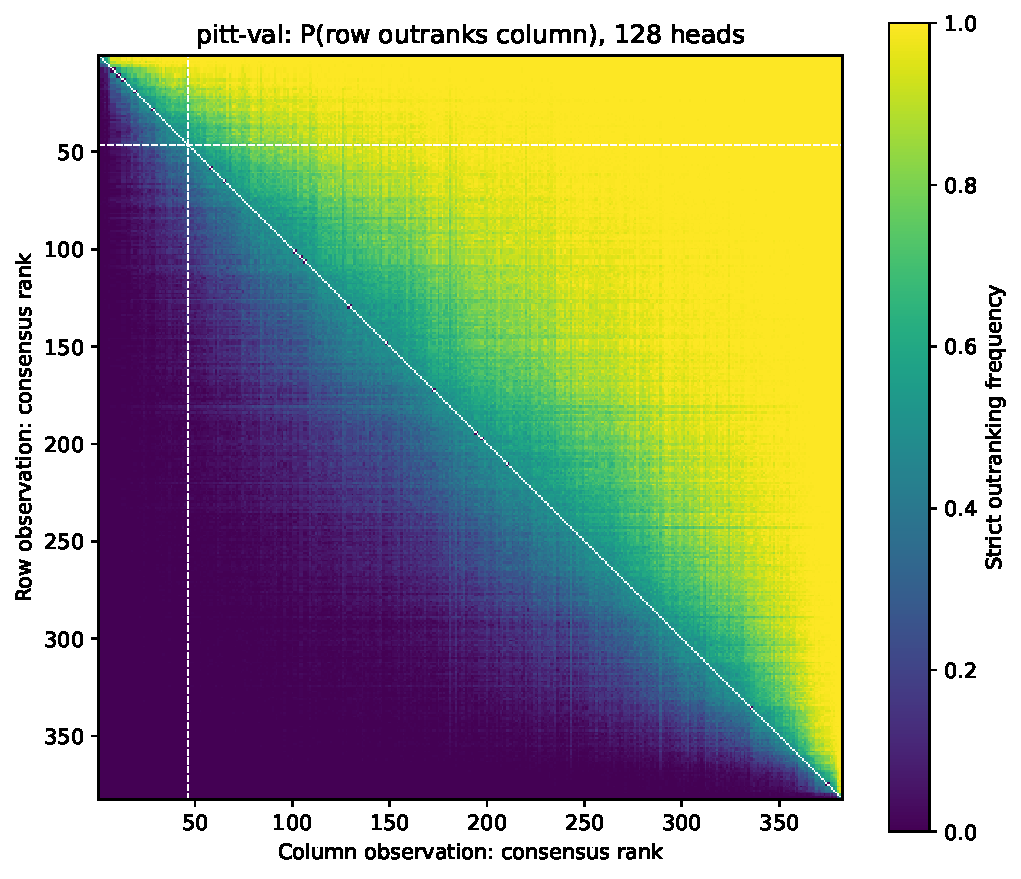
\includegraphics[width=.88\linewidth]{figures/point_4_pitt-val_pairwise_heatmap.pdf}
\caption{Validation pairwise outranking frequencies for all 382 observations, ordered by the certified consensus.}
\label{fig:val-pairwise}
\end{figure}
\clearpage
\begin{figure}[H]
\centering
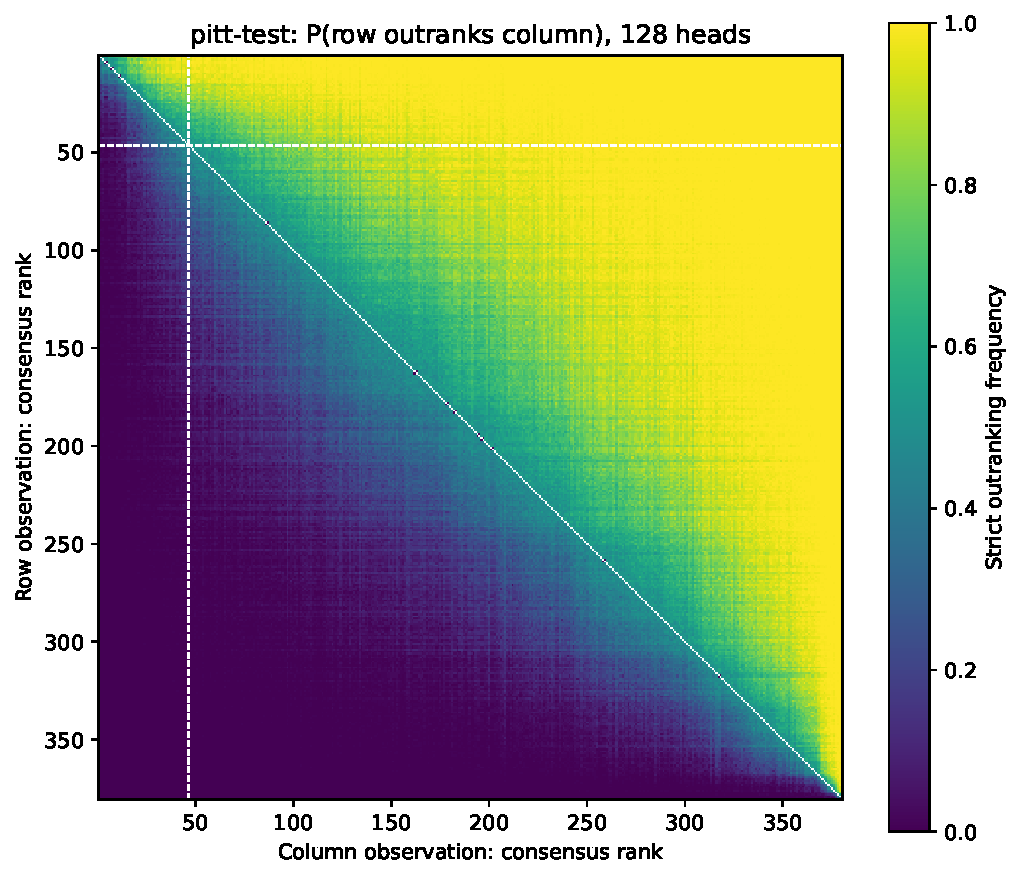
\includegraphics[width=.88\linewidth]{figures/point_4_pitt-test_pairwise_heatmap.pdf}
\caption{Test pairwise outranking frequencies for all 380 observations, ordered by the certified consensus.}
\label{fig:test-pairwise}
\end{figure}
\clearpage
\begin{figure}[H]
\centering
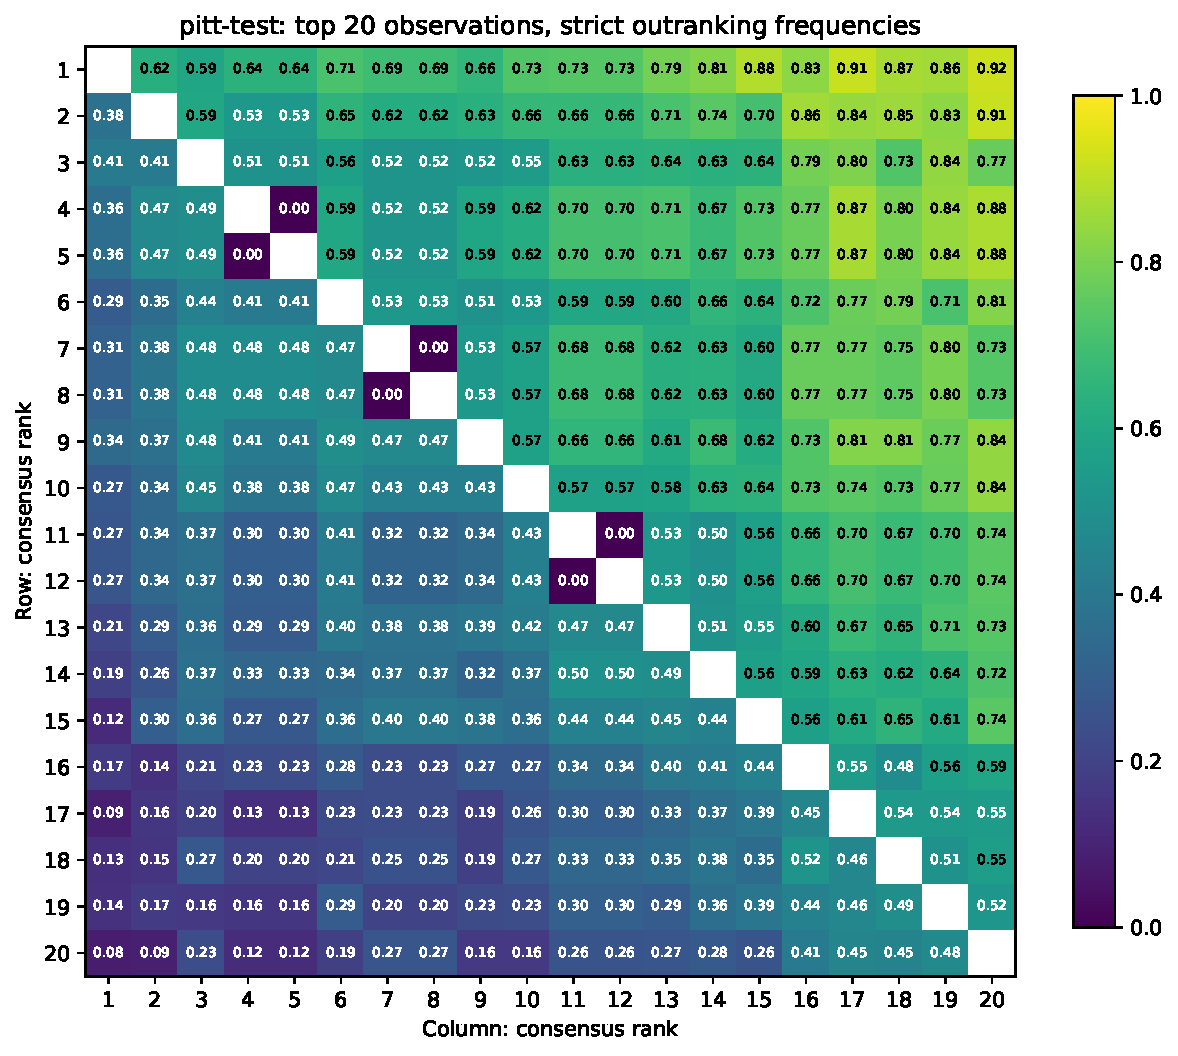
\includegraphics[width=1\linewidth]{figures/point_4_pitt-test_top20_heatmap.pdf}
\caption{Test top-20 consensus positions. Values are strict outranking frequencies rounded to two decimals. The zero-valued opposite cells at positions 4/5, 7/8 and 11/12 correspond to exact score ties across all heads.}
\label{fig:test-top20}
\end{figure}

\end{document}
